\documentclass[a4paper,11pt,oneside,]{article}
\usepackage{
  %fancyvrb,
  %color,
  graphbox,
  hyperref,
  amsmath,
  graphicx,
  xcolor,
}
%\usepackage{palatino}
\usepackage{fbb}
% \usepackage{pygments}
% \usepackage{minted}
\usepackage[a4paper,text={16.5cm,25.2cm},centering]{geometry}
\usepackage{lipsum}
\usepackage[labelformat=simple,position=top]{subcaption}
% \renewcommand\thesubfigure{\alph{subfigure})}
\hypersetup{
  pdfauthor = {Srdjan Sarikas},
  pdftitle={Intracellular Receptors},
  colorlinks=TRUE,
  linkcolor=blue,
  citecolor=red,
  urlcolor=green
}
% \newcommand{\Regions}{{\texttt{Regions}}}

%\setlength{\parindent}{0pt}
%\setlength{\parskip}{1.2ex}

\title{Intracellular Receptors \\ {\small Materials and Methods: Analysis and Processing}}

\author{Srdjan}
\date{\today}

\begin{document}
\maketitle

%<<echo=False>>=
%import matplotlib.pyplot as plt
%import numpy as np
%import pandas as pd
%from islets import load_regions
%@

\section{General pipeline}

A typical experiment involving imaging of pancreatic slices in our lab concerns a single field of view
showing up to hundreds of cells, in a recording of at least several, often dozens, gigabytes.
Current tools (ImageJ, \dots) rely on loading the recording, or its part, into memory, for viewing, analysis, and processing.
It also requires laborious and long human engagement.
We have developed a set of interdependent tools to automatize as much as possible the analysis pipeline (see fig.~\ref{fig:pipeline}). 
The crucial elements of our pipeline are the following:
\begin{itemize}
\item (Semi-)automatic detection of regions of interest (ROIs);
\item Transformation of ROI time traces into standard score ("z-score") and correction for filtering distortion;
\item Quantification of the phenotype for each ROI in terms of the distribution of events of different durations.
\end{itemize}

Our toolset is inspired and relies on CaImAn \cite{giovannucci2019caiman}, a similar package developed for the purposes in neuroscience research.


\begin{figure}[h]
\centering
\includegraphics[width=\textwidth,trim=1.5cm 1.5cm 15mm 15mm,clip]{figures/pipeline.pdf}
\caption{
\label{fig:pipeline}
An illustration of our processing and analysis pipeline:
({\it i})  From a full movie, we calculate the mean (or other statistic) across all frames.
({\it ii}) We pass the mean image through a band-pass filter and define ROIs by detecting local peaks.
({\it iii}) We save ROIs with all the important information (time traces, ROI coordinates, movie statistics, recording frequency, pixel size, etc.).
({\it iv}) Traces contain features at very different timescales---with different timescales presumably important for different cell types. We collect them into separable events for analysis.
}
\end{figure}

\subsection{(Semi-)Automatic Detection of Regions of Interest}

Once imported, a recording is stored as a 3-dimensional ($T{\times}x{\times}y$) numpy array \cite{2020NumPy-Array}.
When the recording is stable, obtaining a mean image, or any other statistic over frame, is rather trivial. 
In case there is horizontal movement, it can be corrected for by aligning the frames to a template. 
For this we use the functionality present in CaImAn \cite{giovannucci2019caiman}, except that high frequency recordings need to be rebinned to some moderate frequency (a few Hz), before correcting, in order to reduce the noise level. 
Once the translation offsets are obtained, we use them to correct the recording in original frequency.

To define regions of interest, we blur the representative image by a kernel of the size we expect cells to be, and at the scale double of that.
The difference between these two images represents a band-pass filter of the original, where the local intensity variation are emphasized (fig.\ref{fig:regions}).
We then pass through all pixels where the value of the filtered image is positive (or larger than a small positive threshold), and for each pixel we search for a local peak in its vicinity. 
All the pixels that lead to the same local peak are then grouped into a single ROI.

As we are mainly interested in islet cells, we choose the kernel size to approximately correspond to $10\mu$m, the characteristic length scale of the islets cells.
If the pixel size is unknown, the choice of kernel is up to the person running the scripts.


\begin{figure}[t]
\centering
\begin{minipage}{.25\textwidth}
    \vskip 2mm
    {\fontfamily{phv}\selectfont A} 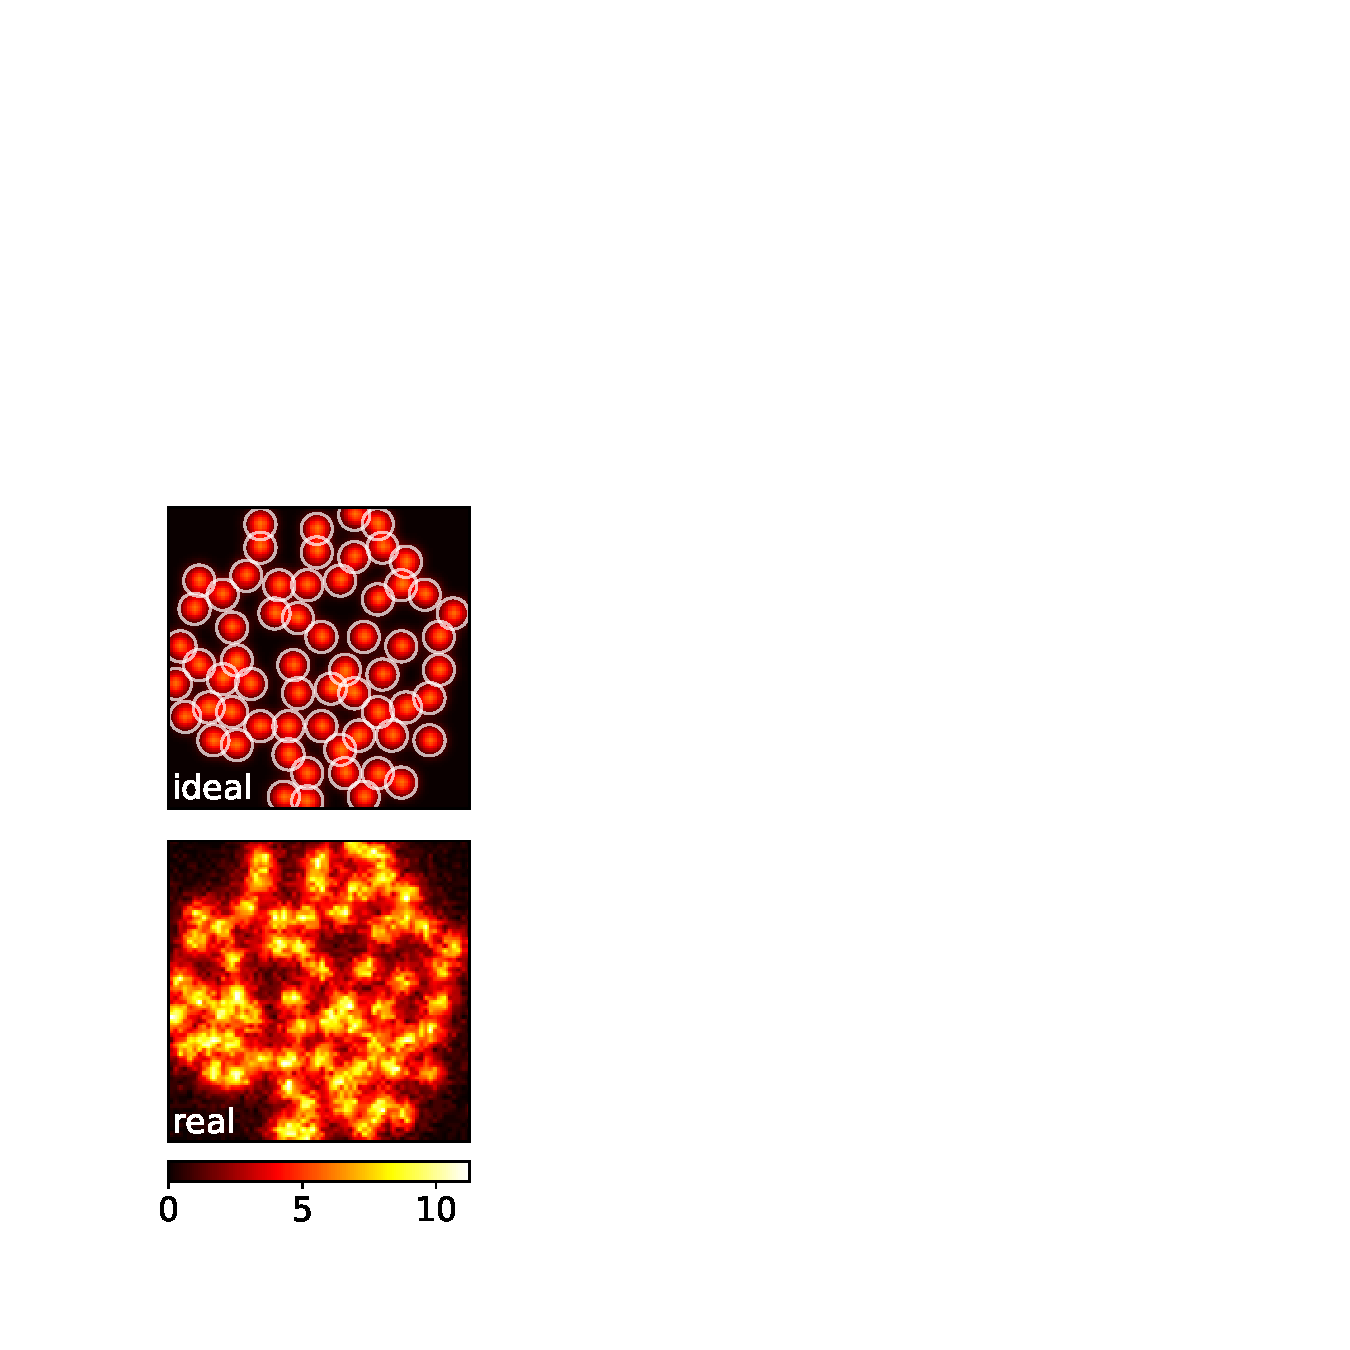
\includegraphics[scale=.5,align=t,trim=25mm 15mm 130mm 72mm, clip]{figures/regions_ideal_real.pdf}\\
    {\fontfamily{phv}\selectfont C} 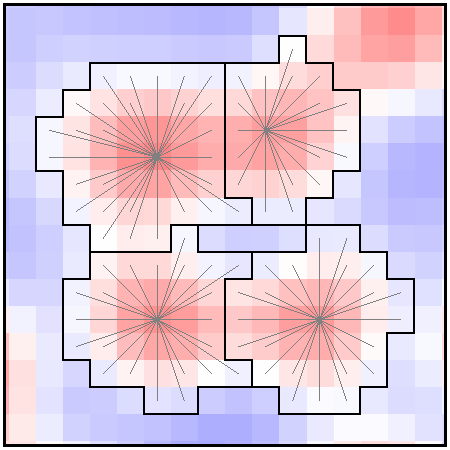
\includegraphics[scale=.33,align=t,trim={-5mm -1mm -1mm -10mm}]{figures/regions_stars.pdf}
\end{minipage}
\begin{minipage}{.6\textwidth}
    \vskip 7mm
    {\fontfamily{phv}\selectfont B} 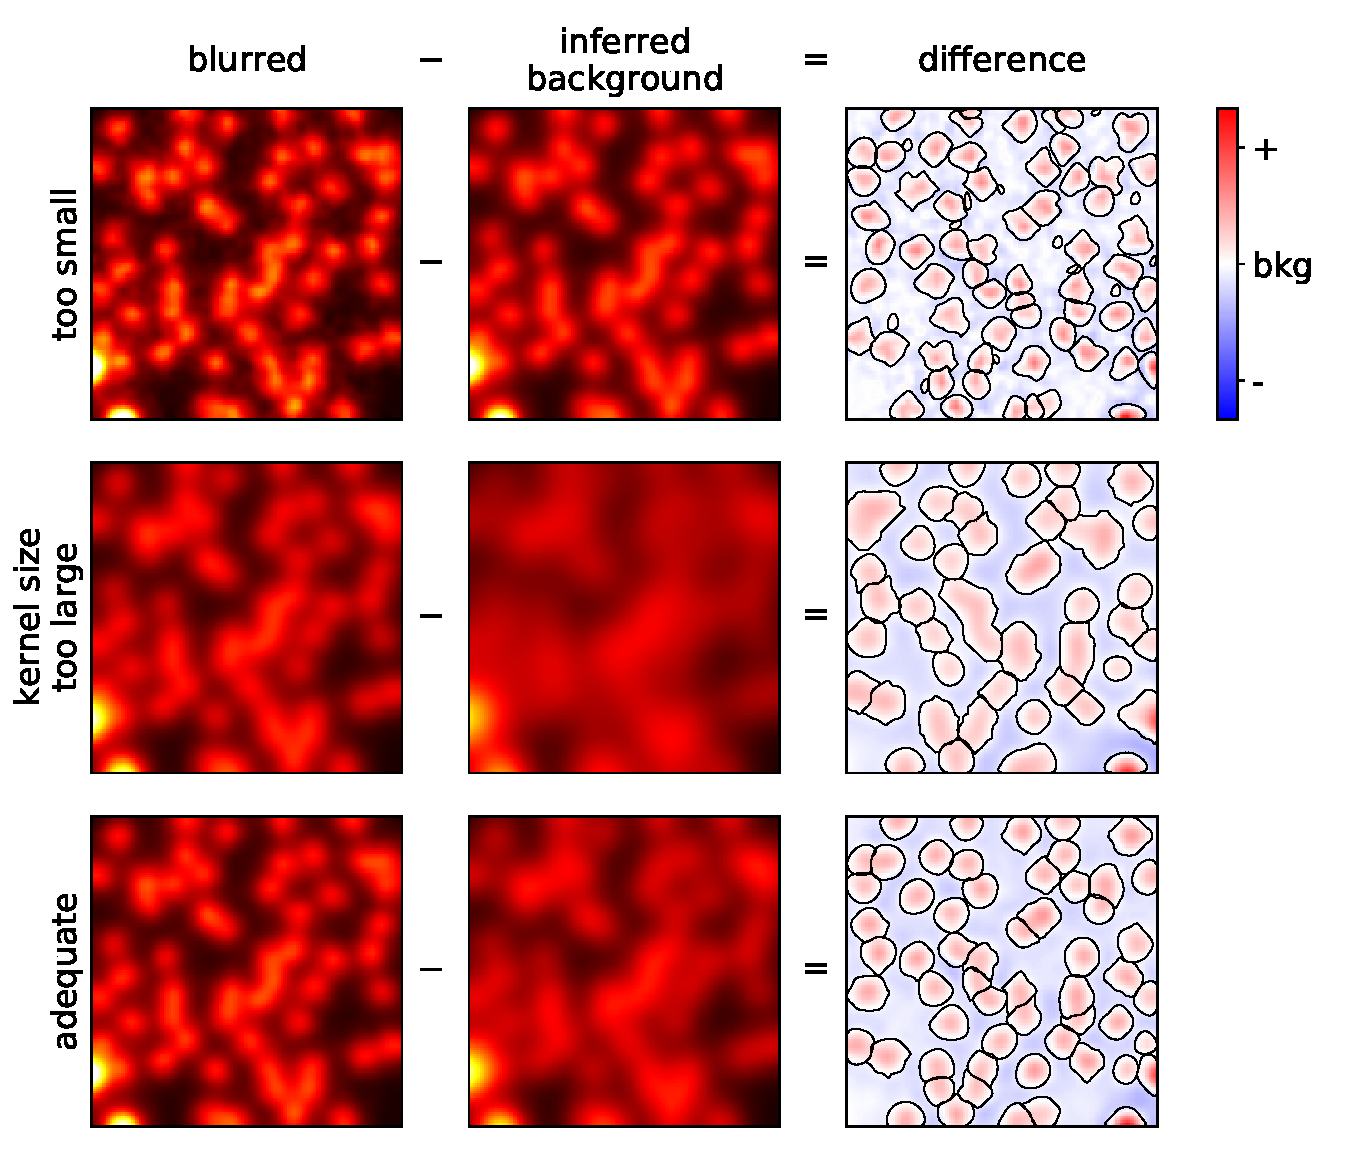
\includegraphics[scale=.5,align=t,trim=10mm 15mm 20mm 15mm, clip]{figures/regions_kernels.pdf}
\end{minipage}
\caption{
(A) Computationally created template $64{\times}64$ image with uniform spherical cells, and with Poisson noise added.
(B) Band-pass filtering of the "realistic" image from A, with different kernel sizes, for denoising  ({\it left}), and  for approximating background  ({\it middle}).
The difference is the filtered image, used to construct ROIs ({\it right}).
The size of the kernel determines the approximate size of the ROIs obtained.
In thick red contours we emphasize misidentified ROIs; the dots indicate the real locations of the cells.
(C) Each ROI is constructed by explicitly searching for a closest peak in intensity. A pixel can only be part of a single ROI.
\label{fig:regions}}
\end{figure}

Representative image can be a mean over all frames or any other statistic.
In addition our code supports standard deviation, mean and standard deviation of the first derivative of the movie, and a ``robust maximum'' of the movie.
As "robust maximum`` we define a very high percentile of the set absolute values of a set, essentially a value close to its maximum, by default it is 10th largest. 
We avoid the maximum as a means to make analysis robust to outliers.
This statistic is sensitive to cells which fire extremely rarely during a recording, so that the mean of those pixels is negligible.
By default, we choose an average of the mean and high percentile as a representative image for band-pass filtering and ROI extraction.

\subsection{Trace processing}

\subsubsection{$z$-score and filtering}

In an ideal detector, recording a time trace of a single pixel in absence of any signal would consist of independent values of the number of photons detected during the dwell time.
The values ($x$) are then distributed according to the Poisson distribution, with standard deviation ($\sigma_1$) being equal to the square root of the mean $\mu_1$, $\sigma_1=\sqrt{\mu_1}$.

% It is often useful to transform a set of numbers to a new 
A transformation to a new variable %$x\rightarrow z$
$$z=\frac{x-\mu}{\sigma}$$
is called {\it standard transformation}, and the new variable standard score or $z$-score (fig.\ref{fig:z_score}). It recasts the initial quantity $x$ in the units of standard deviation from the expected mean. A noisy trace in $z$ spends $95$\% of the time between $-2$ and $2$, and $99.7$\% between $-3$ and $3$. Probability of $z>3$ is very small $p<0.0013$, which is why it is often considered a threshold value for pointing out the outliers.

In general, the mean slow component needs to be inferred, typically by low-pass filtering. Throughout this project, we use cascaded second-order section (sos) filtering, implemented in \verb|scipy.signal| module~\cite{2020SciPy-NMeth}. The cut-off frequency $f_{cut}$ of a filter determines the timescale of the events that can be detected in $z$-score. 

\begin{figure}[t]
    \centering
    \begin{minipage}{.49\textwidth}
        {\fontfamily{phv}\selectfont A} 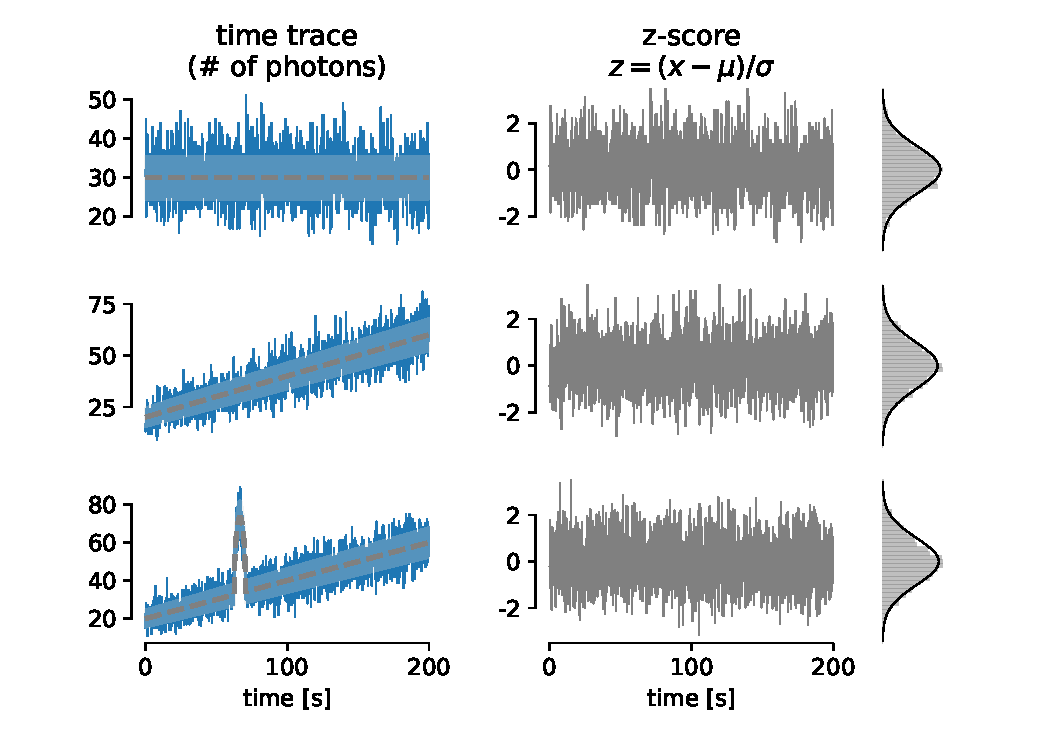
\includegraphics[scale=.5,trim=13mm 0 0 0,clip,align=t]{figures/z_score_1.pdf}
    \end{minipage}
    \begin{minipage}{.49\textwidth} 
        {\fontfamily{phv}\selectfont B} \includegraphics[scale=.5,trim=15mm 30mm 0 0,clip,align=t]{figures/z_score_2.pdf}
        {\fontfamily{phv}\selectfont C} 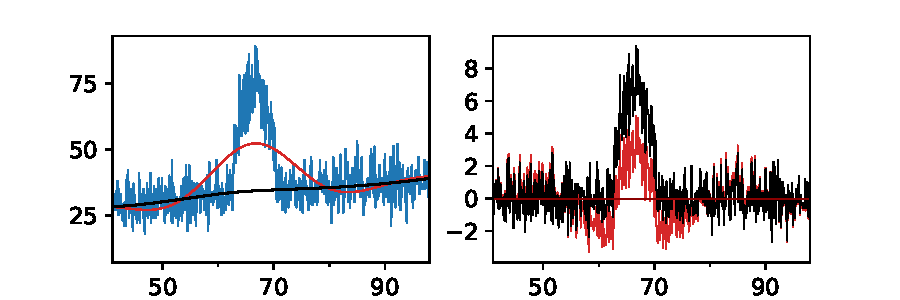
\includegraphics[scale=.48,trim=5mm 0mm 0 0,clip,align=t]{figures/z_score_3.pdf}
    \end{minipage}
    \caption{
    (A) \emph{Left}: Simulated traces with Poisson noise (blue) around different means (grey) with different temporal features. The shaded area represents one standard deviation interval around mean. 
    \emph{Right}: Irrespective of the shape of the mean, z-score transformation behaves exactly as a Gaussian variable with zero mean and unit standard deviation.\\
    (B) The values of $z$-scores depends on the reference. In subfigure (A), the reference curves are known, but in general they need to be inferred, typically by low-pass filtering. The cut-off frequency $f_{cut}$ of a filter determines the timescale of the events that can be detected in $z$-score. If filtered with too high cut-off (orange), the resulting smooth curve follows too closely the trace and the event is not visible in $z$. With $f_{cut}=1/50$~Hz, the resulting $z$-score has obvious outliers ($z\geq 3$), visible both in trace and in the histogram.\\
    (C) Zoom to the indicated regions form B. The original (blue) and the filtered trace and $z$-score (red), and the filtered trace and $z$-score corrected for distortion (black).
    \label{fig:z_score}
    }
\end{figure}


\paragraph{Correcting for the filtering distortion} 
Fast Fourier transform naturally distorts signals, but the inferred $z$-score can be used to correct for it. We constructed an iterative filtering algorithm, where at each iteration, we neglect the outlier values of the original trace, substitute them with the values of the slow component, and reapply the filter. At each iteration, the distortion is less prominent, increasing the $z$-score.
In fig.~\ref{fig:z_score}C, we show the result after 10 iterations, though we find three iterations is a more conservative choice, and a reasonable compromise between results and computing time.


\paragraph{ROI traces}
All above refers also to a sum of pixel traces, but, crucially, not to their mean. A sum of two pixels $a$ and $b$ ($x=x_a+x_b$), with means $\mu_a$ and $\mu_b$, would have a standard deviation as expected $\sigma = \sqrt{\mu} = \sqrt{\mu_a+\mu_b}$. But, if we were to consider the average $\tilde x = x/2$, standard deviation would be $\sqrt{2}$ times smaller $\tilde \sigma = \sigma/\sqrt{2}$.
Therefore, when calculating $z$ score for a ROI trace, we always consider the sum, rather than the average trace of the underlying pixels. When we visualize traces, we show them averaged, only to keep the scales comparable.

The same reasoning holds for rebinning a single trace, where the resulting trace, rebinned by a factor of $n$,  has a standard deviation $\sqrt{n}$ times smaller than the original.


\begin{figure}[t]
 \centering
 \includegraphics[trim=25mm 0 20mm 10mm, clip,scale=0.9]{figures/mean_vs_var.pdf}
 \caption{
 {\it Left}: Regions of interest for the two experiments recorded using the raw photon-counting mode ({\it top}, used for {\color{red} Fig.1} in the main text), and the standard mode with large gain ({\it bottom}). Pixels which had at least 10 saturated values are shown in green. In thick red contours we emphasize ROIs with at least 30 green pixels used to emphasize the influence of saturation (see below).
 \\
 For each recording, we filter the ROI traces at $1$s ({\it middle}) and $10$s ({\it right}) to separate the trace into slow and fast component. For each ROI we then randomly choose $100$ values of the slow component together with the variance of the fast component from a window around the same timepoint, with window size the same as the timescale.
 \\
 In agreement with our assumptions, the variances and the means are linearly dependent, and in the case of raw photon counts, the dependence is exactly 1 (solid diagonal line $\sigma^2=\mu$). In the standard mode, the dependence is still linear, yet with a slope larger than one (dashed orange line). Points above the bulk in this view are due to windows with larger variance, and presumably connected with activity (at the appropriate timescale). Points below the bulk are due to undervariate windows. They are concentrated at high values and are due to saturated pixels. In the lower right plot we emphasize this fact by showing the points from saturated ROIs in red.
 }
 \label{fig:mean_vs_var}
\end{figure}



\subsubsection{Realistic detectors}
All{\color{red}?} the experiments discussed in this manuscript were recorded on a Leica setup with Hybrid detector in photon counting mode.
In this case, we see no significant departure from our assumption of Poisson distribution.
Even with non-unit gain, the linear dependence between variance and mean remains, though the slope is different from $1$ (fig.~\ref{fig:mean_vs_var}).

Other types of detectors introduce additional sources of noise other than Poisson (e.g. thermal), but, mostly it is still dominated by Poisson in our experience, at least as long as the values between neighboring pixels and frames are independent.


\subsection{Identification of Events}

Traces contain features spanning orders of magnitude in time: from tens of miliseconds, to tens of minutes. 
We aim to investigate how do events at these different timescales interact and a connection between them and the islets' environment.
For this, we devised an algorithm based on sequential filtering, followed by .
In the first step, we perform a sequential filtering of the traces at timescales starting from $0.5$s, and increasing by a factor of $\sqrt[4]{2}$,  $\tau = \{2^{-1}, 2^{-3/4}, 2^{-1/2}, 2^{-1/4},\dots\}$, until the timescale of the longest event we are interested (and in any case it makes no sense to filter at timescale comparable to the length of the experiment itself).
At each timescale, we transform the trace to $z$-score, and identify regions where $z>3$ as {\it candidate events}. 

An event is characterized by the start time ($t_0$), it's maximal height, and the width at the half of the height ({\it halfwidth}, $\delta t$), which is our measurement of it's duration.
For simplicity, we define end time as $t_{\rm end} = t_0+\delta t$, although events arguably last much longer after the intensity drops at half of the peak.

\begin{figure}[t]

 \centering
%  \newgeometry{textwidth=20cm}
 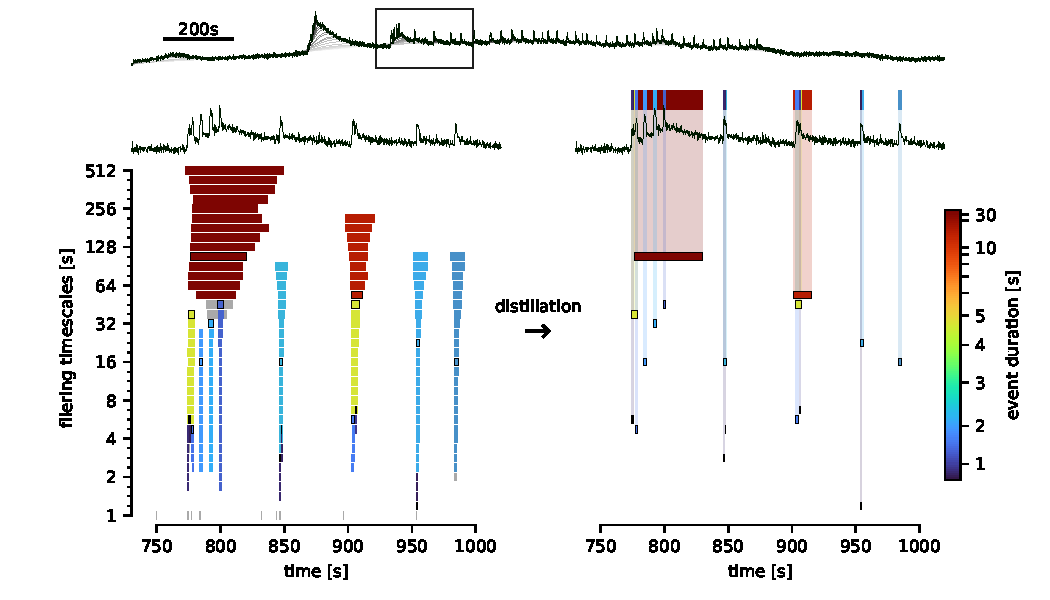
\includegraphics[trim=12mm 0 0mm 0mm, scale=0.9]{figures/evdist.pdf}
 \caption{(A) Example of a trace (black) and slow components in sequential filtering (shades of gray). % Square indicates the regions shown in B and C. 
 (B) Close-up view of the indicated small region from (A) and a representation of all candidate events in that region detected through sequential filtering.
 Each bar represents an event. Vertical position corresponds to the timescale at which the event was detected, the horizontal boundaries correspond to beginning and end time.
 In grey we show events that are deemed false positives, because they are detected at too few filtering timescales.
 Others events belong to groups of similar events which are then considered real; we show a boundary around the bar of the event closest to the one finally distilled. 
 It's time boundaries are set to median of the whole group, and the color indicates its halfwidth.
 (C) Distillation greatly removes redundancies and false positive candidates. Only robust events are selected for further analysis (see text for details). 
 In the top part we represent the distilled events at single height, in a more compact view.
 We choose a color code (mapping to a hill curve) which is nearly linear up to a few seconds, to emphasize the color difference at the timescales most interesting for our analysis.
 }
 \label{fig:evdist_demo}
\end{figure}



If an event is real, it will be detected at multiple timescales, and will start around the same time and will have approximately same halfwidth.
We specify a tolerance of 20\% of the halfwidth as to whether two candidate events should be considered equal; if their start and end times are within 20\% of the halfwidth, they are considered cognates, having arisen due to the same real event. 
For a set of cognates, we estimate the start and end time of the real underlying event as a median over the set.
If the resulting estimate for the halfwidth is larger than 2s, we require that a set consists of at least 4 candidate events (corresponding to event being detectable when filtered at timescales that differ at least two-fold).
For shorter events, we require only that an event is not unique to a single timescale.

We also neglect events that last less than $3$ time frames, as well as those too close to the beginning or end of the recording (within $\delta t/2$), which we ascribe to artefacts from zero-padding for the filtering. 
We term this procedure event {\it distilling} (see fig.~\ref{fig:evdist_demo}).





\section{Analyses}
\subsection{El Toro}
\subsection{Isradipine}
\subsection{Low Ca}
\subsection{etc}

\newpage

\bibliographystyle{plain}% E-Life prefers apa
\bibliography{matmet}


\end{document}
